
\item In the figure below, the switches \( S_1 \) and \( S_2 \) are closed simultaneously at \( t = 0 \) and a current starts to flow in the circuit. Both the batteries have the same magnitude of the electromotive force (emf) and the polarities are as indicated in the figure. Ignore mutual inductance between the inductors. The current \( I \) in the middle wire reaches its maximum magnitude \( I_{\text{max}} \) at time \( t = \tau \). Which of the following statements is (are) true?
\begin{center}
    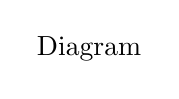
\begin{tikzpicture}
        \node {Diagram};
    \end{tikzpicture}
\end{center}
    \begin{tasks}(2)
        \task \( I_{\text{max}} = \frac{V}{2R} \)
        \task \( I_{\text{max}} = \frac{V}{4R} \)
        \task \( \tau = \frac{L}{R} \ln 2 \)
        \task \( \tau = \frac{2L}{R} \ln 2 \)
    \end{tasks}
    
    \begin{solution}
        Considering the left loop with \( S_1 \), the characteristic time constant for an RL circuit is given by \( \tau = \frac{L}{R} \).
    The current \( I \) will reach its maximum value when the inductor is fully 'charged', which occurs after a time period of \( \tau \).
    The growth of current in an RL circuit can be modeled as:
        \begin{align*}
            I(t) &= \frac{\varepsilon}{R} \left(1 - e^{-\frac{R}{L}t}\right),
        \end{align*}
        where \( \varepsilon \) is the emf of the battery. When \( t = \tau \), we have:
        \begin{align*}
            I_{\text{max}} &= \frac{\varepsilon}{R} \left(1 - e^{-\frac{R}{L}\tau}\right) = \frac{\varepsilon}{R} \left(1 - e^{-1}\right).
        \end{align*}
        Thus, for the given system, \( \tau = \frac{L}{R} \ln 2 \) is the correct expression for the time constant, making option (C) the
    correct answer. Options (A), (B), and (D) do not accurately describe \( I_{\text{max}} \) or the time constant \( \tau \) for this
    circuit.
    \end{solution}